\documentclass[
	10pt,								% globale Schriftgröße
	parskip=half-,						% setzt Absatzabstand hoch
	paper=a4,							% Format
	english,ngerman,					% lädt Sprachpakete
	]{scrartcl}							% Dokumentenklasse

% //////////////////// Pakete laden ////////////////////
\usepackage{amsmath}			% MUSS vor fontspec geladen werden
\usepackage{mathtools}			% modifiziert amsmath
\usepackage{amssymb}			% mathematische symbole, für \ceckmarks
\usepackage{amsthm}				% für proof
\usepackage{mathrsfs}			% für \mathscr
\usepackage{latexsym}
\usepackage{marvosym}				% für Lightning

\usepackage{fontspec} 			% funktioniert nur mit den neueren Compilern z.B. XeLaTeX
\usepackage{microtype}			% für bessere Worttrennung
\usepackage[ngerman]{babel} 	% Spracheinstellung
\usepackage{csquotes}
\usepackage{lmodern}			% verändert verwendete Schriftart, damit sie weniger pixelig ist

\usepackage{verbatim}
\usepackage{listings}			% Für Quellcode

\usepackage{graphicx}
\usepackage{tabularx}			% für Tabellen mit gleicher Spaltenbreite und automatischen Umbrüchen
\usepackage{fullpage}
\usepackage{multirow}			% für multirow in tabulars
\usepackage{rotate}
\usepackage[cmyk,table]{xcolor} % um Farben zu benutzen, kann mehr als das Paket color
\usepackage[					% Verlinkungen
	colorlinks,					% farbige Schrift, statt farbiger Rahmen
	linktocpage,				% verlinkt im Abb.Verzeichnis Seitenzahl statt Bildunterschrift
	linkcolor=blue				% setzt Farbe der Links auf blau
	]{hyperref}					% nur für digitale Anwendungen, url = "http://www.example.com"
\usepackage{url}				% für Webadressen wie e-mail usw.: "\url{http://www.example.com}"

\usepackage{enumerate}			% für versch. Aufzählungezeichen wie z.B. a)
\usepackage{xspace}				% folgt ein Leerzeichen nach einem \Befehl, wird es nicht verschluckt.
\usepackage{cancel}				% für das Durchstreichen u.a. in Matheformeln mit \cancel
\usepackage{float}              % zum Forcieren der Position von figure-Umgebungen

% zum Zeichnen (u.a. von Graphen)
\usepackage{fp}
\usepackage{tikz}
\usetikzlibrary{tikzmark}			% für \tikzmark{toRemember}
\usetikzlibrary{positioning}	% verbesserte Positionierung der Knoten
\usetikzlibrary{automata}		% für Automaten (GTI)
\usetikzlibrary{arrows}
\usetikzlibrary{shapes}
\usetikzlibrary{decorations.pathmorphing}
\usetikzlibrary{decorations.pathreplacing}
\usetikzlibrary{decorations.shapes}
\usetikzlibrary{decorations.text}

% //////////////////// Syntaxhighlighting ////////////////////
\lstloadlanguages{Python, Haskell, [LaTeX]TeX, Java}
\lstset{
   basicstyle=\footnotesize\ttfamily,	% \scriptsize the size of the fonts that are used for the code
   backgroundcolor = \color{bgcolour},	% legt Farbe der Box fest
   breakatwhitespace=false,	% sets if automatic breaks should only happen at whitespace
   breaklines=true,			% sets automatic line breaking
   captionpos=t,				% sets the caption-position to bottom, t for top
   commentstyle=\color{codeblue}\ttfamily,% comment style
   frame=single,				% adds a frame around the code
   keepspaces=true,			% keeps spaces in text, useful for keeping indentation
							% of code (possibly needs columns=flexible)
   keywordstyle=\bfseries\ttfamily\color{codepurple},% keyword style
   numbers=left,				% where to put the line-numbers;
   							% possible values are (none, left, right)
   numberstyle=\tiny\color{codegreen},	% the style that is used for the line-numbers
   numbersep=5pt,			% how far the line-numbers are from the code
   stepnumber=1,				% nummeriert nur jede i-te Zeile
   showspaces=false,			% show spaces everywhere adding particular underscores;
							% it overrides 'showstringspaces'
   showstringspaces=false,	% underline spaces within strings only
   showtabs=false,			% show tabs within strings adding particular underscores
   flexiblecolumns=false,
   tabsize=1,				% the step between two line-numbers. If 1: each line will be numbered
   stringstyle=\color{orange}\ttfamily,	% string literal style
   numberblanklines=false,				% leere Zeilen werden nicht mitnummeriert
   xleftmargin=1.2em,					% Abstand zum linken Layoutrand
   xrightmargin=0.4em,					% Abstand zum rechten Layoutrand
   aboveskip=2ex, 
}

\lstdefinestyle{py}{
   language=Python,
}
\lstdefinestyle{hs}{
   language=Haskell,
}
\lstdefinestyle{tex}{
	language=[LaTeX]TeX,
	escapeinside={\%*}{*)},     % if you want to add LaTeX within your code
	texcsstyle=*\bfseries\color{blue},% hervorhebung der tex-Schlüsselwörter
	morekeywords={*,$,\{,\},\[,\],lstinputlisting,includegraphics,
	rowcolor,columncolor,listoffigures,lstlistoflistings,
	subsection,subsubsection,textcolor,tableofcontents,colorbox,
	fcolorbox,definecolor,cellcolor,url,linktocpage,subtitle,
	subject,maketitle,usetikzlibrary,node,path,addbibresource,
	printbibliography},% if you want to add more keywords to the set
     numbers=none,
     numbersep=0pt,
     xleftmargin=0.4em,
}

\lstdefinestyle{java}{
	language=Java,
	extendedchars=true,		% lets you use non-ASCII characters;
   						% for 8-bits encodings only, does not work with UTF-8
}

\lstdefinelanguage[x64]{Assembler}     % add a "x64" dialect of Assembler
   [x86masm]{Assembler} % based on the "x86masm" dialect
   % with these extra keywords:
   {morekeywords={CDQE,CQO,CMPSQ,CMPXCHG16B,JRCXZ,LODSQ,MOVSXD, %
                  POPFQ,PUSHFQ,SCASQ,STOSQ,IRETQ,RDTSCP,SWAPGS, %
                  rax,rdx,rcx,rbx,rsi,rdi,rsp,rbp, %
                  r8,r8d,r8w,r8b,r9,r9d,r9w,r9b}
}					% for 8-bits encodings only, does not work with UTF-8

\lstdefinestyle{c}{
	language=c,
	extendedchars=true,		% for 8-bits encodings only, does not work with UTF-8
}

% //////////////////// eigene Kommandos ////////////////////
\newcommand\FU{Freie Universität Berlin\xspace}% benötigt package xspace
\newcommand\gdw{g.\,d.\,w.\xspace}
\newcommand\oBdA{o.\,B.\,d.\,A.\xspace}
\newcommand{\Eu}{\texteuro}
\newcommand\N{\mathbb{N}\xspace}
\newcommand\Q{\mathbb{Q}\xspace}
\newcommand\R{\mathbb{R}\xspace}
\newcommand\Z{\mathbb{Z}\xspace}
\newcommand\ohneNull{\ensuremath{\backslash\lbrace 0\rbrace}}% \{0}
\let\dhALT\dh	% Schreibt Befehl \dh in \dhALT um
\renewcommand\dh{d.\,h.\xspace}	%renew überschreibt command \dh
\newcommand\Bolt{\;\text{\LARGE\raisebox{-0.3em}{\Lightning}\normalsize}\xspace}% Blitz
\newcommand\zz{\ensuremath{\raisebox{+0.25ex}{Z}% zu zeigen
			\kern-0.4em\raisebox{-0.25ex}{Z}%
			\;\xspace}}
\newcommand{\from}{\ensuremath{\colon}}
\newcommand{\floor}[1]{\lfloor{#1}\rfloor}
\newcommand{\ceil}[1]{\lceil{#1}\rceil}
 \renewcommand{\L}{\ensuremath{\mathcal{L}}\xspace}
 \renewcommand{\P}{\ensuremath{\mathcal{P}}\xspace}
 \newcommand{\NL}{\ensuremath{\mathcal{N}\kern-0.2em\mathcal{L}}\xspace}
 \newcommand{\NP}{\ensuremath{\mathcal{NP}}\xspace}

% //////////////////// Mathefunktionen ////////////////////
\DeclareMathOperator{\Landau}{\mathcal{O}}
\DeclareMathOperator{\True}{True}
\DeclareMathOperator{\False}{False}

% //////////////////// eigene Theoreme ////////////////////
\newtheorem{theorem}{Satz}
\newtheorem{corollary}[theorem]{Folgerung}
\newtheorem{lemma}[theorem]{Lemma}
\newtheorem{observation}[theorem]{Beobachtung}
\newtheorem{definition}[theorem]{Definition}
\newtheorem{Literatur}[theorem]{Literatur}
% konfiguriert proof
\makeatletter
\newenvironment{Proof}[1][\proofname]{\par
  \pushQED{\qed}%
  \normalfont \topsep6\p@\@plus6\p@\relax
  \trivlist
  \item[\hskip\labelsep
%         \itshape
        \bfseries
    #1\@addpunct{.}]\ignorespaces
}{%
  \popQED\endtrivlist\@endpefalse
}
\makeatother

% //////////////////// eigene Farben ////////////////////
\let\definecolor=\xdefinecolor
\definecolor{FUgreen}{RGB}{153,204,0}
\definecolor{FUblue}{RGB}{0,51,102}

\definecolor{middlegray}{rgb}{0.5,0.5,0.5}
\definecolor{lightgray}{rgb}{0.8,0.8,0.8}
\definecolor{orange}{rgb}{0.8,0.3,0.3}
\definecolor{azur}{rgb}{0,0.7,1}
\definecolor{yac}{rgb}{0.6,0.6,0.1}
\definecolor{Pink}{rgb}{1,0,0.6}

\definecolor{bgcolour}{rgb}{0.97,0.97,0.97}
\definecolor{codegreen}{rgb}{0,0.6,0}
\definecolor{codegray}{rgb}{0.35,0.35,0.35}
\definecolor{codepurple}{rgb}{0.58,0,0.82}
\definecolor{codeblue}{rgb}{0.4,0.5,1}

% //////////////////// eigene Settings ////////////////////

\textheight = 230mm		% Höhe des Satzspiegels / Layouts
\footskip = 10ex			% Abstand zw. Fußzeile und Grundlinie letzter Textzeile
\parindent 0pt			% verhindert Einrückung der 1. Zeile eines Absatzes
\setkomafont{sectioning}{\rmfamily\bfseries}% setzt Ü-Schriften in Serifen, {disposition}
\graphicspath{ {./src/} } 
\usepackage{hyperref}

\newcommand{\dozent}{Volker Roth}
\newcommand{\tutor}{Oliver Wiese}
\newcommand{\tutoriumNo}{02\\Materialien: Latex, VSC, Skript}
\newcommand{\ubungNo}{05}
\newcommand{\veranstaltung}{Rechnersicherheit}
\newcommand{\semester}{SoSe 21}

% /////////////////////// BEGIN DOKUMENT /////////////////////////
\begin{document}
% /////////////////////// BEGIN TITLEPAGE /////////////////////////
\begin{titlepage}
	\subject{\dozent}
	\title{\veranstaltung, \semester}
	\subtitle{\Large Übung \ubungNo\\ \large\vspace{1ex} TutorIn: \tutor\\ Tutorium \tutoriumNo}
	\author{\studenten}
	\date{\normalsize \today}
\end{titlepage}

\maketitle								% Erstellt das Titelblatt
\vspace*{-10cm}							% rückt Logo an den oberen Seitenrand
\makebox[\dimexpr\textwidth+1cm][r]{	%rechtsbündig und geht rechts 1cm über Layout hinaus
	
\includegraphics[width=0.4\textwidth]{src/fu_logo} % fügt FU-Logo ein
}
% /////////////////////// END TITLEPAGE /////////////////////////

\vspace{7cm}							% Abstand
\rule{\linewidth}{0.8pt}				% horizontale Linie

% /////////////////////// Task 1 /////////////////////////
\section{Shoulder surfer meets Markov}
\begin{enumerate}[(a)]
    % /////////////////////// a /////////////////////////
    \item {\itshape Give  an  algorithm  with  observed  digits  (less  than  4)  as  input  and  outputs  three likely PINs.}
    \begin{enumerate}[1.]
        \item We assume that we always observe only the first digit of the PIN.
        \item First we preprocessed the Markov model that we expect to get thought a file. We expect this form of representation, because we defined it like that in the last exercise sheet. The following snipped shows the form we expect of a Markov model:
        \lstinputlisting[language=python,linerange={13-24}]{src/u5/markov_model.txt}
        Here is the Markov model after we preprocessed it. Now it is ordered from highest possibility that that char is taken to lowest:
        \lstinputlisting[language=python,linerange={44-55}]{src/u5/processed_markov_model.txt}
        And here is the code on how we did it:
        \lstinputlisting[language=python,linerange={5-40}]{src/u5/guess_pin.py}
        

\newpage
        \item After that we ran the following function. It takes the Markov model, the processed Markov model, the observed digit, the number of PINs we want to get and an accuracy int as input. The function is greedy and always takes the next digit with the highest possibility, which is quite easy, because of the preprocessing we did with the Markov model. After it found more PINs than 'num\_of\_output\_pins' it drops the PIN with the lowest total possibility. 
        \lstinputlisting[language=python,linerange={42-71}]{src/u5/guess_pin.py}

        
    \end{enumerate}
    

    % /////////////////////// b /////////////////////////
    \item {\itshape Discuss the efficiency and success rate of your algorithm.}
   \begin{itemize}
       \item The efficiency and success rate of your algorithm dependents on the accuracy variable. As our algorithm has three for loops, its efficiency is accuracy$^{3}$. 
       \item Accuracy should/ can not be higher than the length of the alphabet, that is 10. So if we choose accuracy = 10 we basically try each possible combination. 
       \item However with accuracy = 10 our algorithm always succeeds and returns the most likley 3 PINs. When we lower the accuracy we might not get the best 3 PINs, but in our tests half of that (5) seemed sufficient. What follows is a picture of the 3 most likely PINs of the Markov model from the RockYou dataset and how different accuracy values affect these PINs.
       
       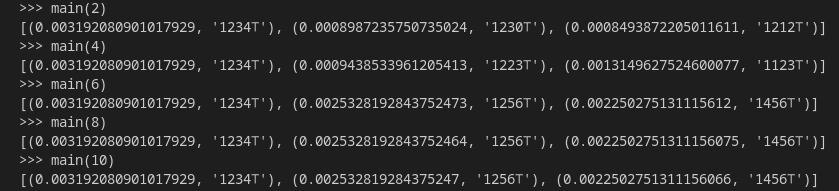
\includegraphics[width=\linewidth]{src/u5/output.png}

   \end{itemize}

\newpage
    % /////////////////////// c /////////////////////////
    \item {\itshape Revisit the first-order Markov model from the previous assignment. What are your guesses if the adversary observes only a one.}
   \begin{itemize}
       \item The expected input Markov model (snipped):
       \lstinputlisting[language=python,linerange={8-20}]{src/u5/u4_markov_model.txt}
       
       \item After the preprocessing (snipped):
       \lstinputlisting[language=python,linerange={20-55}]{src/u5/p_u4_markov_model.txt}
       
       \item The output:
       
       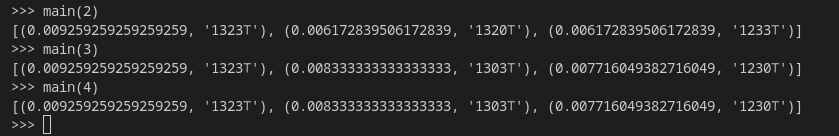
\includegraphics[width=\linewidth]{src/u5/output2.png}
   \end{itemize}
   
    
\end{enumerate}

% /////////////////////// Task 2 /////////////////////////
\section{Shoulder surfer meets Markov II (Bonus)}
\begin{enumerate}[(a)]
    % /////////////////////// a /////////////////////////
    \item {\itshape Create a markov model of 4- and 6-digit PINs based on the RockYoudata set using Python. You can either filter them by yourself or use the dataset ofMarkert et al.}
    \begin{itemize}
        \item After some preprocessing of the RockYou dataset and error filtering (like in the last exercise sheet) we just filtered the dataset with a regex. Snipped of the code:
       \lstinputlisting[language=python,linerange={50-57, 62-67}]{src/u5/rockyou_to_4-6PIN.py}
        Snippet of the filtered dataset:
       \lstinputlisting[language=python,linerange={0-20}]{src/u5/4_6_PIN.txt}

    \end{itemize}
    
    % /////////////////////// b /////////////////////////
    \item {\itshape Implement your above algorithm in Python.}
    \begin{itemize}
        \item First we load the dataset and add the bot and top symbol to every PIN
        \lstinputlisting[language=python,linerange={10-15}]{src/u5/dataset_to_markov_model.py}
\newpage        
        \item Then we count the occurrences of every char in the alphabet:
        \lstinputlisting[language=python,linerange={17-33}]{src/u5/dataset_to_markov_model.py}
        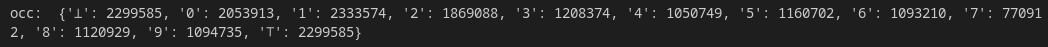
\includegraphics[width=\linewidth]{src/u5/output_occ.png}
        
        \item After that we create the alphabet for the Markov model (the edges) and count the occurrences of these chars (edges) as well:
        \lstinputlisting[language=python,linerange={36-41}]{src/u5/dataset_to_markov_model.py}
        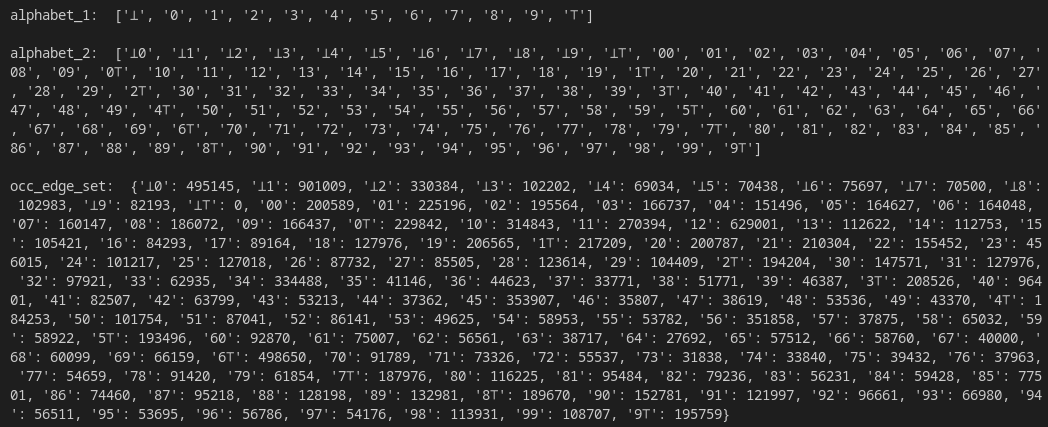
\includegraphics[width=\linewidth]{src/u5/output_occ_2.png}
        
        \item And at last we calculate the Markov modell with these occurrences:
        \lstinputlisting[language=python,linerange={43-50}]{src/u5/dataset_to_markov_model.py}

    \end{itemize}

    % /////////////////////// c /////////////////////////
    \item {\itshape Evaluate  your  algorithms.  What  is  the  advantage  of  your  algorithms compared to a random guess?}
    \begin{itemize}
        \item If we use the Markov model like in task 1. and output three likely PINs when we observe one digit. We get the following results: 
        
        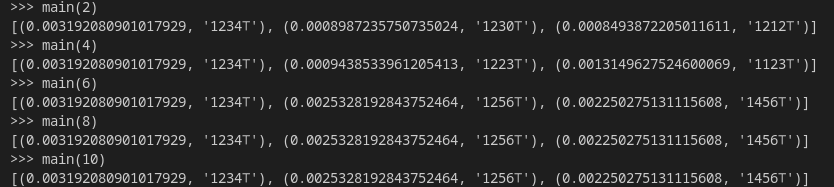
\includegraphics[width=\linewidth]{src/u5/output3.png}
        \\ These PINs are better than a random guess, as they are much more likely to occur. A random guess would have the probability of $\frac{1}{10^{3}}$ = 0.001, which is just a third compared to our most likely PIN: ~ 0.0032.  
        
    \end{itemize}

\end{enumerate}


% /////////////////////// Task 3 /////////////////////////
\section{Follow up}


Please read Sections 4.1 and 4.2 of the paper3and answer the following questions:
\begin{enumerate}[(a)]
    
    % /////////////////////// a /////////////////////////
    \item {\itshape What are the differences to the algorithm from the lecture?}
    
    
    % /////////////////////// b /////////////////////////
    \item {\itshape Why do you think Algorithm 1 is different?}


    % /////////////////////// c /////////////////////////
    \item {\itshape What are the consequences for storage and runtime?}

\end{enumerate}


Compare algorithm from the lecture to algorithms their algorithms:
\begin{enumerate}[(a)]

    % /////////////////////// a /////////////////////////
    \item {\itshape partial\_size1(current\_length, level)}
    
    % /////////////////////// b /////////////////////////
    \item {\itshape partial\_size2(current\_length, prev\_char, level)}
    
    % /////////////////////// pseudo c  /////////////////////////
    \item {\itshape Is a table size of maxlength · maxlevel enough?}

    \begin{enumerate}[1.]
        \item In the lecture l stands for level / rank, while in the note, it stands for the length of a password
        \item In the lecture $p_1$ or probability($e_1$) stands for the probability of an char / edge, while in the note they use $\nu$ (Ny) 
        \item For the probability of a path / password, they use the symbol $\theta$ (Theta)
        \item They don't show how to save the save the information, which is goatherd with partial\_size1. While algorithm 1 does show that the information gets stored in a table.
        \item The partial\_size1 algorithm supposes that the Markov model is of order 1. While the Algorithm 1 does not.
        \item The partial\_size1 and 2 algorithms only allow passwords with a fixed (same) length, while the algorithm from the lecture allows passwords of different sizes.
        \item Also the table size of max\_length · max\_level is not enough. In the paper for partial\_size1 they argue that a 2D-Array of size l times number of levels should be sufficient. That is the case for partial\_size1, as each probability is independent of one another. But not for partial\_size2, because it works for Markov models order 1, thus it loses the independence of probability and a larger table will be needed.
    \end{enumerate}


\end{enumerate}
\end{document}